\chapter{LODでの公開機構}
本章ではLODでの公開機構について述べる.

\section{スキーマとURI}
// TODO:

\subsection{スキーマ定義}
// TODO:

\subsection{URIエンドポイント}
// TODO:

\section{アクセス制御}
先に述べたように,ゴオルシェアではLinked Dataのアクセス権限を指定することができず,自動的にすべてのデータが誰でも閲覧できる状況にあった.
しかし研究室など限られた組織内で使うには,アクセス権限のあるユーザーのみが閲覧できる仕組みが必要である.
そこで現状では,アカウント単位でのアクセスコントロール機能があるRDFストアであるStardogを用いて,表1に示すような,プロジェクトの段階に応じたアクセス制御機構を実装中である.
具体的には\ref{img:permission_table}に示すように,(1)プロジェクトが個人的な構想段階である初期場合,(2)組織内限定で共有される段階,(3)外部発表後に外部公開する段階,(4)オープンライセンスで公開し,組織横断的な協働を志向する段階,の4段階を想定し,各段階に応じたアクセス制御機構を想定している.
プロジェクトの段階が進んでいくにつれて,公開したいタスクが増えていくと考えられる.
ただし,より具体的な下層の葉に近いタスクは,段階が進んだとしても公開に適さない場合が多いと考えられる.
そこで,タスクツリーからユーザが公開したいタスクのみを部分的に選択できるようなインターフェースも必要となる.
このような公開箇所の選択機構についても,現在実装中である.

\begin{figure}[t]
	\begin{center}
		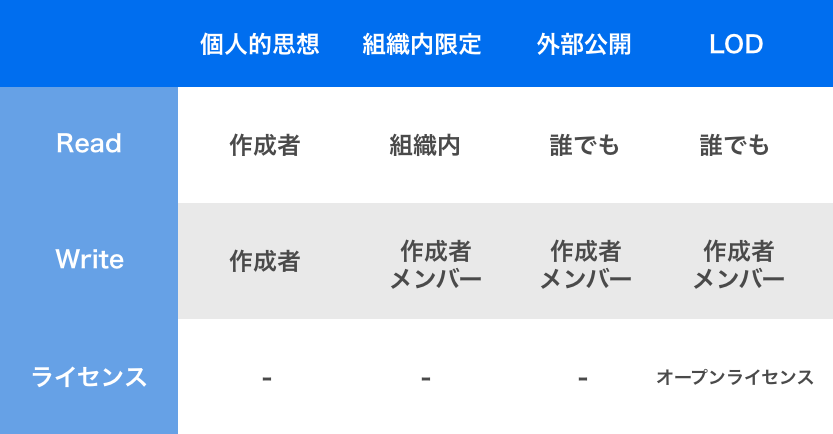
\includegraphics[width=0.9\linewidth]{assets/img/permission_table.png}
		\caption{アクセス権限}
		\label{img:permission_table}
	\end{center}
\end{figure}

\section{実装手法}
// TODO: 具体的な実装手法
